Here we briefly describe the various routines for generating initial models
for the main MAESTRO problems and how the initial model is used to initialize
both the base state and the full Cartesian state.

\MarginPar{I think it would be a good idea to mention some where in here that MAESTRO outputs info that's useful to check --dr of base state and dr of the input file, which should be the same at the finest level; and Maximum HSE Error, which should be some small number.}

\section{Creating the Model Data from Raw Data}\label{Sec:Creating the Model Data from Raw Data}
\label{sec:initial_models_main}

We have found that for the best performance, the MAESTRO initialization procedure should be given model data with the same resolution as the base state resolution, $\Delta r$.  For planar problems, $\Delta r = \Delta x$.  For multilevel planar problems, we use $\Delta r$ equal to $\Delta x$ at the finest resolution.  For spherical problems we set $\Delta r = \Delta x/\mathtt{drdxfac}$.  We generate our initial model either analytically or from raw data,
 $\rho^{\raw}, T^{\raw}, p^{\raw}$, and $X^{\raw}$.  
Here is the raw data file for each test problem:
\begin{eqnarray}
{\tt test2} & \rightarrow & \mathrm{none-it~ is~ generated~ analytically} \nonumber \nonumber \\
{\tt test\_convect} & \rightarrow & \mathrm{none-it~ is~ generated~ analytically} \nonumber \nonumber \\
{\tt wdconvect} & \rightarrow & {\tt initial\_models/kepler/model\_6.e8.raw} \nonumber \\
{\tt spherical\_heat} & \rightarrow & \mathrm{none-it~ is~ generated~ analytically} \nonumber \\
{\tt xrb} & \rightarrow & {\tt initial\_models/xrb/sorted\_xrb.raw} \nonumber
\end{eqnarray}

We use a fortran subroutine
to interpolate the raw data, yielding the model data, $\rho^{\model},
T^{\model}, p^{\model}$, and $X^{\model}$.  The fortran subroutine
then uses an iterative procedure to modify the model data so that it
is thermodynamically consistent with the {\tt MAESTRO} equation of
state (EOS), and also satisfies our chosen hydrostatic equilibrium
(HSE) discretization,
\begin{equation}
\frac{p_r - p_{r-1}}{\Delta r} = \frac{\rho_r + \rho_{r-1}}{2}g_{r-\myhalf},\label{HSE Discretization}
\end{equation}
to a user defined tolerance.  Here are the fortran subroutines for each test problem:
\begin{eqnarray}
{\tt test2} & \rightarrow & {\tt initial\_models/test2/init\_1d.f90} \nonumber \\
{\tt test\_convect} & \rightarrow & {\tt initial\_models/test2/init\_1d.f90} \nonumber \\
{\tt wdconvect} & \rightarrow & {\tt initial\_models/kepler/init\_1d.f90} \nonumber \\
{\tt spherical\_heat} & \rightarrow & {\tt initial\_models/spherical/init\_1d.f90} \nonumber \\
{\tt xrb} & \rightarrow & {\tt initial\_models/xrb/init\_1d.f90} \nonumber
\end{eqnarray}
The model data is not generated at run-time - it must be generated in
advance of running any MAESTRO examples.  The inputs file should point
to the file containing the model data.

\section{Creating the Initial Data from the Model Data}
In {\tt base\_state.f90}, using the subroutine {\tt
  init\_base\_state} (which is actually a terrible name since we
are computing 1D initial data, which is not quite the same thing 
as the base satte), we set the initial
data $\rho^{\init}, T^{\init}, p^{\init}$ and $X^{\init}$ equal to the
model data.  Then, we set $p^{\init},h^{\init} =
p,h(\rho^{\init},T^{\init},X^{\init})$ through the EOS.  Note that 
we overwrite the existing value of $p^{\init}$ but this should not change
the value since we called 
$p^{\model} = p^{\model}(\rho^{\model},T^{\model},X^{\model})$ at the end of the
initial model generation routines in 
\S~\ref{Sec:Creating the Model Data from Raw Data}.

For multilevel planar problems, we generate
initial data at the non-finest levels by using linear interpolation
from the two nearest model points (see Figure \ref{Fig:Multilevel
  Initialization}).  Note that the initial data is not in HSE nor is
it thermodynamically consistent on non-finest cells.  We will enforce
these on the base state and full state later.
%%%%%%%%%%%%%%%%%%%%%%%%%%%%%%%%%
\begin{figure}[tpb]
\centering
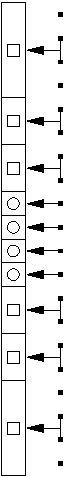
\includegraphics[width=0.4in]{\figpath/multilevel_init}\hspace{0.2in}
\begin{minipage}[b]{5.0in}
\caption[Multi-level initial model initialization]
 {Multilevel Initialization.  The data from the initial model
  is represented by the dots on the right.  The initial data at the
  finest level is represented by the circles.  The initial data at
  non-finest levels is represented by the squares.  We copy data from
  the dots directly into the circles.  We use linear interpolation
  using the two nearest points to copy data from the dots to the
  squares.\vspace{2em}}
\end{minipage}
\label{Fig:Multilevel Initialization}
\end{figure}
%%%%%%%%%%%%%%%%%%%%%%%%%%%%%%%%%

We deal with the edge of the star by tracking the first coarse cell 
in which the density falls below {\tt base\_cutoff\_density}.  We note 
the radius of this cell center, and the values of $\rho$, $\rho h$, $X_k$, 
$p$, and $T$ in this cells.  Then, at every level, if current cell-center 
is above this radius, we set the state equal to this stored state.  This 
ensures a consistent treatment of the edge of the star at all levels.

\section{Creating the Base State and Full State}\label{Sec:Creating the Base State and Full State}

Given $p^{\init}, \rho^{\init}, T^{\init},$ and $X^{\init}$, this
section describes how the base state ($\rho_0$ and $p_0$) and full
state ($\rho, h, X$, and $T$) are computed.  The base state is, general, not
simply a direct copy of the initial model data, since we require that
$\rho_0 = \overline\rho$.  Additionally, we require thebase state to
be HSE according to equation (\ref{HSE Discretization}), and that the full
state is thermodynamically consistent with $p_0$.  Overall we do:
\begin{enumerate}
\item Fill $\rho^{\init}, h^{\init}, X^{\init}$, and $T^{\init}$ onto a 
  multifab to obtain the full state $\rho, h, X$, and $T$.
\item If {\tt perturb\_model} = T, a user-defined perturbation is
  added.  This routine should make sure that the EOS is called so that
  there is some sense of thermodynamic consistency.
\item Set $\rho_0 = \overline\rho$.
\item Compute $p_0$ using {\tt enforce\_HSE}.
\item Compute $T,h = T,h(\rho,p_0,X_k)$.
\item Set $(\rho h)_0 = \overline{(\rho h)}$.
\item Compute $\overline{T}$.  Note that we only use $\overline{T}$ as
  a diagnostic and as a seed for EOS calls.
\end{enumerate}
Now $\rho_0 = \overline\rho$, the base state is in HSE, and the full
state is thermodynamically consistent with $p_0$.

\subsection{Coarse-Fine {\tt enforce\_HSE} Discretization}\label{Sec:Coarse-Fine HSE Discretization}
When integrating the HSE discretization upward, we must use a different
differencing procedure at coarse-fine interfaces.  Figure~\ref{fig:ctof} shows
the transition from coarse (level $l-1$) to fine (level $l$), with the zone
center indices noted.  
\begin{figure}[t]
\centering
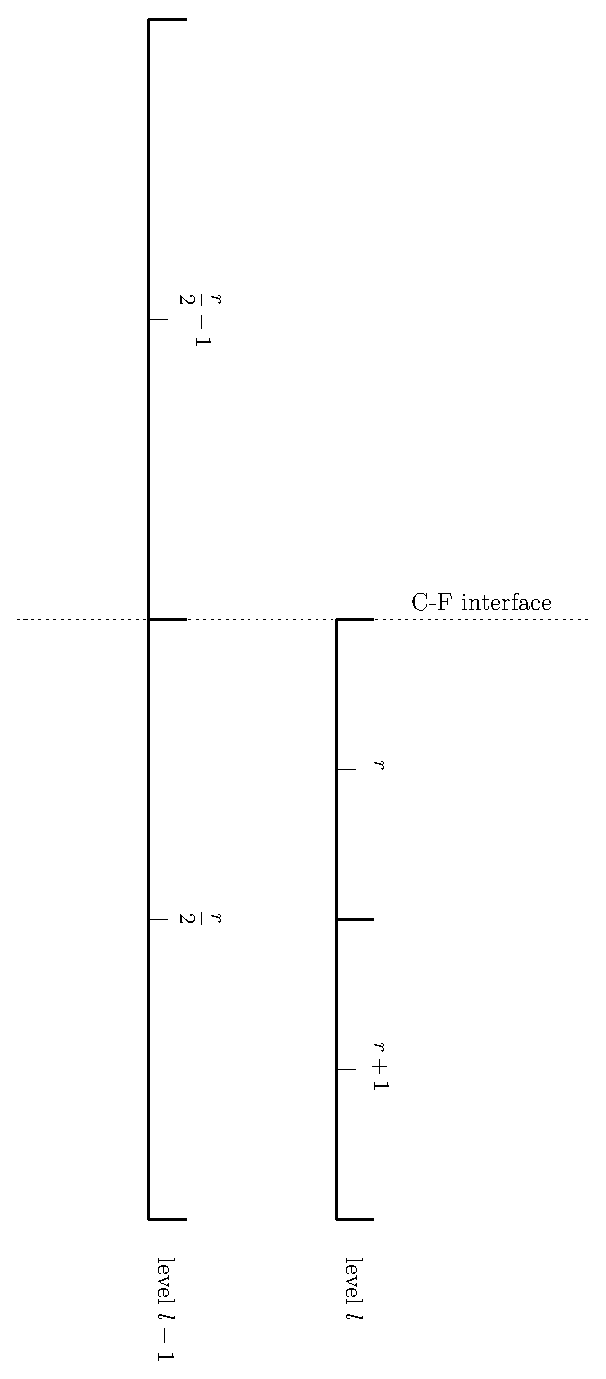
\includegraphics[width=2.5in,angle=90]{\figpath/ctof}
\caption{\label{fig:ctof} A coarse-fine interface in the 1-d base state}
\end{figure}

To find the zone-centered pressure in the first fine zone, $p_r^l$, from
the zone-centered pressure in the coarse zone just below the coarse-fine interface,
$p_{\sfrac{r}{2}-1}^{l-1}$, we integrate in 2 steps.  We allow for a spatially
changing gravitational acceleration, for complete generality.

First we integrate up to the
coarse-fine interface from the coarse-cell center as:
\begin{equation}
\frac{p_{r-\myhalf}^l - p_{\sfrac{r}{2}-1}^{l-1}}{\Delta r^{l-1}/2} = 
  \frac{\rho_{r-\myhalf}^l + \rho_{\sfrac{r}{2}-1}^{l-1}}{2}  \,
  \frac{g_{r-\myhalf}^l + g_{\sfrac{r}{2}-1}^{l-1}}{2} 
\end{equation}
We can rewrite this as an expression for the pressure at the coarse-fine interface:
\begin{equation}
 p_{r-\myhalf}^l = p_{\sfrac{r}{2}-1}^{l-1} + \frac{\Delta r^{l-1}}{8}
  \left(\rho_{r-\myhalf}^l + \rho_{\sfrac{r}{2}-1}^{l-1}\right)
  \left(g_{r-\myhalf}^l + g_{\sfrac{r}{2}-1}^{l-1}\right).
  \label{eq:ctoi}
\end{equation}

Next we integrate up from the coarse-fine interface to the fine-cell center:
\begin{equation}
\frac{p_r^l - p_{r-\myhalf}^l}{\Delta r^l/2} = 
  \frac{\rho_r^l + \rho_{r-\myhalf}^l}{2} \,
  \frac{g_r^l + g_{r-\myhalf}^l}{2}
\end{equation}
We can rewrite this as an expression for the pressure at the fine-cell center:
\begin{equation}
p_r^l = p_{r-\myhalf}^l + \frac{\Delta r^l}{8}
  \left(\rho_r^l + \rho_{r-\myhalf}^l\right)
  \left(g_r^l + g_{r-\myhalf}^l\right).
  \label{eq:itof}
\end{equation}
Combining equations \ref{eq:ctoi} and \ref{eq:itof} gives
\begin{eqnarray}
p_r^l = p_{\sfrac{r}{2}-1}^{l-1} &+& 
     \frac{\Delta r^{l-1}}{8} \left(\rho_{r-\myhalf}^l + \rho_{\sfrac{r}{2}-1}^{l-1}\right)
                                \left(   g_{r-\myhalf}^l +    g_{\sfrac{r}{2}-1}^{l-1}\right) \nonumber \\
 &+& \frac{\Delta r^l}{8} \left(\rho_r^l + \rho_{r-\myhalf}^l\right)
                            \left(   g_r^l +    g_{r-\myhalf}^l\right).
\end{eqnarray}
We can simplify using
\begin{equation}
\Delta r^{l-1} = 2\Delta r^l,
\end{equation}
and by interpolating the cell-centered densities to the coarse-fine interface as:
\begin{equation}
\rho_{r-\myhalf}^l = \frac{2}{3}\rho_r^l + \frac{1}{3}\rho_{\sfrac{r}{2}-1}^{l-1}.
\end{equation}
Because we carry both the cell- and edge-centered gravitational accelerations, we
do not need to interpolate $g$ to the interface.
Simplifying, we have
\begin{eqnarray}
p_r^l = p_{\sfrac{r}{2}-1}^{l-1} &+& 
   \frac{\Delta r^l}{4}\left(\frac{2}{3}\rho_r^l + 
                             \frac{4}{3}\rho_{\sfrac{r}{2}-1}^{l-1} \right)
                       \left(   g_{r-\myhalf}^l +    g_{\sfrac{r}{2}-1}^{l-1}\right) \nonumber \\
  &+& \frac{\Delta r^l}{8}\left(\frac{5}{3}\rho_r^l + 
                                  \frac{1}{3}\rho_{\sfrac{r}{2}-1}^{l-1}\right) 
                       \left(   g_r^l +    g_{r-\myhalf}^l\right) \enskip .
\end{eqnarray}
Finally, we note for constant $g$, this simplifies to:
\begin{equation}
p_r^l = p_{\sfrac{r}{2}-1}^{l-1} + 
  \frac{3\Delta r^l g}{4}\left(\rho_{\sfrac{r}{2}-1}^{l-1} + \rho_r^l\right).\label{Coarse-Fine Stencil}
\end{equation}

When integrating across a fine-coarse interface (see Figure~\ref{fig:ftoc}), the proceduce is similar.
\begin{figure}[t]
\centering
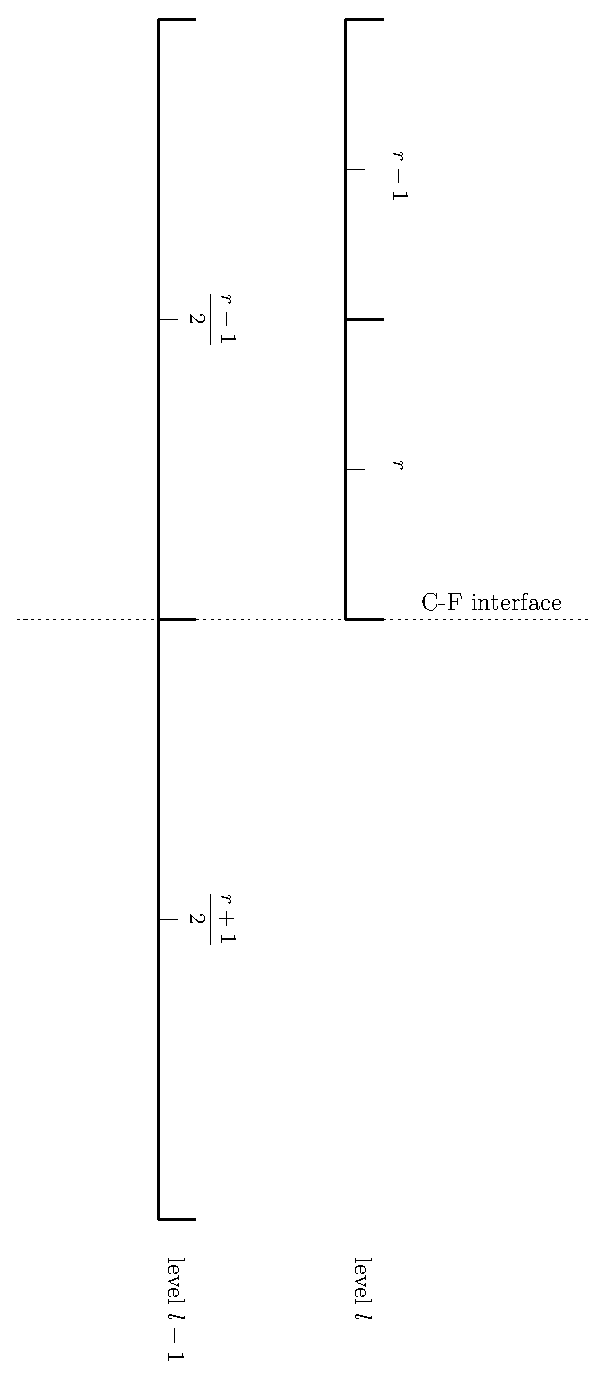
\includegraphics[width=2.5in,angle=90]{\figpath/ftoc}
\caption{\label{fig:ftoc} A fine-coarse interface in the 1-d base state}
\end{figure}
The expression for general gravity becomes:
\begin{eqnarray}
p_{(r+1)/2}^{l-1} = p_{r}^l &+&
   \frac{\Delta r^l}{4}\left(\frac{2}{3}\rho_r^l + 
                             \frac{4}{3}\rho_{(r+1)/2}^{l-1} \right)
                       \left(   g_{(r+1)/2 -\myhalf}^{l-1} +    g_{(r+1)/2}^{l-1}\right) \nonumber \\
  &+& \frac{\Delta r^l}{8}\left(\frac{5}{3}\rho_r^l + 
                                  \frac{1}{3}\rho_{(r+1)/2}^{l-1}\right) 
                       \left(   g_r^l +    g_{(r+1)/2 -\myhalf}^{l-1} \right) \enskip .
\end{eqnarray}
and for spatially-constant gravity, it simplifies to:
\begin{equation}
p_{(r+1)/2}^{l-1} = p_{r}^l + \frac{3\Delta r^l g}{4}\left(\rho_{r}^l+\rho_{(r+1)/2}^{l-1}\right).\label{Fine-Coarse Stencil}
\end{equation}

